\documentclass[11pt,a4paper]{article}

% ── Encoding & fonts ──────────────────────────────────────────────────────────
\usepackage[utf8]{inputenc}
\usepackage[T1]{fontenc}
\usepackage{lmodern}

% ── Page layout ───────────────────────────────────────────────────────────────
\usepackage[top=2.5cm, bottom=2.5cm, left=2.8cm, right=2.8cm]{geometry}

% ── Typography ────────────────────────────────────────────────────────────────
\usepackage{microtype}
\usepackage{setspace}
\onehalfspacing

% ── Math ──────────────────────────────────────────────────────────────────────
\usepackage{amsmath}
\usepackage{amssymb}

% ── Graphics ──────────────────────────────────────────────────────────────────
\usepackage{graphicx}
\usepackage{float}

% ── Tables ────────────────────────────────────────────────────────────────────
\usepackage{booktabs}
\usepackage{array}
\usepackage{tabularx}

% ── TikZ (pipeline diagram) ───────────────────────────────────────────────────
\usepackage{tikz}
\usetikzlibrary{shapes.geometric, arrows.meta, positioning, calc}

% ── Section formatting — black only, no colors ────────────────────────────────
\usepackage{titlesec}
\titleformat{\section}{\large\bfseries}{\thesection}{1em}{}[\titlerule]
\titleformat{\subsection}{\normalsize\bfseries}{\thesubsection}{1em}{}
\titleformat{\subsubsection}{\normalsize\bfseries\itshape}{\thesubsubsection}{1em}{}

% ── Captions ──────────────────────────────────────────────────────────────────
\usepackage[font=small, labelfont=bf, justification=centering]{caption}

% ── Lists ─────────────────────────────────────────────────────────────────────
\usepackage{enumitem}

% ── Hyperlinks — black, no colored boxes ──────────────────────────────────────
\usepackage[colorlinks=false, hidelinks, breaklinks=true]{hyperref}
\usepackage{url}

% ── Header / footer ───────────────────────────────────────────────────────────
\usepackage{fancyhdr}
\pagestyle{fancy}
\fancyhf{}
\renewcommand{\headrulewidth}{0.4pt}
\fancyhead[L]{\small\textit{FusionGuardNet: Audio Deepfake Detection}}
\fancyhead[R]{\small\thepage}

% ── Paragraph spacing ─────────────────────────────────────────────────────────
\setlength{\parskip}{0.45em}
\setlength{\parindent}{0pt}

% ── Custom abstract style ─────────────────────────────────────────────────────
\usepackage{abstract}
\renewcommand{\abstractnamefont}{\normalfont\small\bfseries\scshape}
\renewcommand{\abstracttextfont}{\normalfont\small}

% ─────────────────────────────────────────────────────────────────────────────
\begin{document}

% ── Title block (preprint style) ──────────────────────────────────────────────
\begin{center}

\rule{\linewidth}{1.5pt}\\[0.4em]
{\LARGE\bfseries\scshape
  FusionGuardNet: Audio Deepfake Detection\\[0.35em]
  Using WavLM, Whisper, and Nes2Net
}\\[0.4em]
\rule{\linewidth}{0.8pt}\\[1.0em]

{\small\scshape A Preprint}\\[1.2em]

% Authors
{\normalsize
  Roy Naor$^{1}$ \quad Shani Golomb$^{1}$
}\\[0.5em]

% Supervisors
{\normalsize
  \textit{Supervised by:} Dr.\ Or Anidjar$^{1}$ \quad Dr.\ Roi Yozevitch$^{1}$
}\\[0.7em]

% Affiliation
{\small
  $^{1}$Department of Computer Science, Ariel University, Ariel, Israel
}\\[0.8em]

{\small \today}

\end{center}

\vspace{0.5em}

% ── Abstract ──────────────────────────────────────────────────────────────────
\begin{abstract}
The rapid advancement of generative AI has made synthetic speech increasingly
indistinguishable from natural human voice, posing serious threats to voice
authentication systems and audio-based communication. This project presents
\textbf{FusionGuardNet}, an audio deepfake detection system that combines
complementary representations from two large pre-trained models---\textbf{WavLM}
and \textbf{Whisper}---processed by a \textbf{Nes2Net} classifier.

WavLM captures fine-grained acoustic and speaker-level properties of the audio
signal, while Whisper encodes phonetic and prosodic structure derived from its
speech recognition training. Both encoders are kept fully frozen, and their
768-dimensional frame-level embeddings are combined through a lightweight
learnable weighted fusion layer before being passed to the classifier. This
offline extraction strategy eliminates redundant encoder inference during training
and keeps the system practical on a single GPU.

FusionGuardNet is evaluated on two benchmark configurations. On \textbf{Dataset~1}
(ASVspoof Combined, 10,536 test samples), the model achieves \textbf{99.18\%
accuracy} with a perfectly symmetric error profile of 43 false positives and 43
false negatives. On \textbf{Dataset~2} (ASVspoof-FoR Extended, 17,467 test
samples), it reaches \textbf{99.34\% accuracy} and an \textbf{Equal Error Rate of
0.60\%}, demonstrating stable performance under a broader and more diverse set of
spoofing conditions.

The results support the central hypothesis that fusing acoustic and
phonetic-linguistic representations yields a more robust detector than either
modality alone, while introducing only 1,536 additional trainable parameters over
the single-encoder baseline.

\medskip
\noindent\textit{Keywords:} audio deepfake detection $\cdot$ self-supervised learning
$\cdot$ WavLM $\cdot$ Whisper $\cdot$ feature fusion $\cdot$ Nes2Net $\cdot$ speech anti-spoofing
\end{abstract}

\tableofcontents
\newpage

% ─────────────────────────────────────────────────────────────────────────────
\section{Introduction}

\subsection{Challenges in Audio-Based Deepfake Detection}

Recent advances in generative AI have made it significantly easier to produce
synthetic speech that sounds indistinguishable from a real human voice
\cite{li2024survey,yi2023survey}. Modern text-to-speech (TTS) and voice
conversion (VC) systems can now generate highly convincing audio with minimal
input, enabling an attacker to clone a speaker's voice from only a short
recording \cite{li2025where}. As these technologies continue to improve, the
boundary between authentic and synthetic speech becomes increasingly difficult to
identify using human perception alone.

These audio deepfakes pose a growing security threat
\cite{hong2026vulnerabilities,kamel2025survey}. They can be used to bypass voice
authentication systems, impersonate individuals in phone calls, manipulate
financial transactions through social engineering, or spread disinformation
through fabricated recordings \cite{chandra2025deepfake}. The risk is especially
significant because audio is often treated as a trusted communication channel in
banking, customer service, journalism, legal evidence, and personal communication.

The research community has responded through the ASVspoof challenge series
\cite{kinnunen2019asvspoof,wang2024asvspoof5,liu2023asvspoof2021}, which has run
since 2015 and provides standardized benchmarks and evaluation protocols for
anti-spoofing systems. Building an effective detector is not straightforward:
classical approaches relied on handcrafted features \cite{todisco2017cqcc} and
tend to miss the subtle artifacts that modern synthesis methods introduce, while
generalization to unseen attack types remains a major open challenge
\cite{muller2024harder}.

Fake audio can fail in more than one dimension simultaneously. Some artifacts
are acoustic---unnatural spectral patterns, phase inconsistencies, or waveform
irregularities. Others are phonetic or prosodic---irregular rhythm, weak
co-articulation, or unnatural intonation \cite{nguyen2025linguistic,zhu2024slim}.
A detector relying on a single feature type is vulnerable to synthesis systems
that do not happen to trigger that specific artifact \cite{shi2025benchmarking}.

Our project addresses this challenge by exploring how combining different types of
pre-trained audio representations can produce a more robust and accurate deepfake
detector.

\subsection{Project Goals: Improving Spoofing Classification Using Pre-trained Models}

The main goal of this project is to build a system that reliably distinguishes
between real and synthetic speech and validate it on two established public
benchmark configurations. Rather than designing handcrafted features or training
from scratch, we leverage large pre-trained models \cite{chen2022wavlm,
radford2023whisper} that have already learned rich speech representations from
massive audio data.

A key design decision is the use of \textbf{offline feature extraction}: all
audio representations are extracted and saved to disk before training begins.
This cleanly separates the costly encoding step from the iterative training loop,
dramatically reduces GPU memory pressure, and makes it practical to experiment
with different classifier architectures without re-running large encoder inference.

The end result is a complete detection pipeline trained and evaluated across two
dataset configurations: \textbf{ASVspoof 2019 LA} \cite{kinnunen2019asvspoof}
combined with \textbf{ASVspoof5 (2024)} \cite{wang2024asvspoof5} as Dataset~1,
and an extended version adding \textbf{Fake-or-Real (for-norm)}
\cite{abdeldayem2024fakeorreal} as Dataset~2.

\subsection{Our Contribution: Integrating Whisper with WavLM in the Nes2Net Architecture}

Our main contribution is the design and implementation of \textbf{FusionGuardNet},
which combines \textbf{WavLM} \cite{chen2022wavlm} and \textbf{Whisper}
\cite{radford2023whisper} to analyze the same audio from two complementary
perspectives. WavLM captures low-level acoustic signal patterns, while Whisper
encodes phonetic and prosodic structure. Both representations are extracted
offline, combined through a learnable weighted fusion layer, and passed into a
shared \textbf{Nes2Net} \cite{liu2025nes2net} classifier.

Both encoders remain fully frozen during training. Only the fusion layer and the
Nes2Net backbone are updated, keeping the trainable parameter count small and
preventing catastrophic forgetting. WavLM and Whisper both produce
768-dimensional frame-level embeddings, so the two sequences can be fused without
any additional projection layer.

On Dataset~1, the system achieves \textbf{99.18\% test accuracy} with a
perfectly symmetric error profile (FP\,=\,43, FN\,=\,43). On Dataset~2, it
reaches \textbf{99.34\% accuracy} and an \textbf{EER of 0.60\%}.

% ─────────────────────────────────────────────────────────────────────────────
\section{Related Work}

\subsection{From Classical Methods to Pre-trained Representations}

\textbf{Spoofing} refers to the deliberate use of synthesized, replayed, or
voice-converted speech to deceive an automatic speaker verification system. Early
anti-spoofing systems relied on handcrafted features \cite{todisco2017cqcc}
combined with classical classifiers. As neural TTS improved \cite{li2024survey,
li2025where}, these fixed representations became insufficient and the field moved
toward deep learning \cite{yi2023survey}.

The most effective direction has been large self-supervised models pretrained on
vast natural speech corpora \cite{li2024survey,elkheir2025comprehensive}, which
generalize better to unseen synthesis methods \cite{muller2024harder,
ahmadiadli2025beyond}. Two such models form the backbone of our approach.

\textbf{WavLM} \cite{chen2022wavlm} is developed by Microsoft and trained with a
masked speech prediction task applied to noise-mixed utterances, forcing it to
build robust acoustic representations. It is built on the wav2vec~2.0 framework
\cite{baevski2020wav2vec}, using a CNN waveform encoder followed by a Transformer
stack with Gated Relative Position Bias. Unlike HuBERT \cite{hsu2021hubert} or
wav2vec~2.0, WavLM's denoising pre-training objective makes its representations
particularly robust to signal-level perturbations. The variant we use,
\texttt{microsoft/wavlm-base-plus}, produces frame-level embeddings of dimension
\textbf{768} at 20\,ms resolution \cite{chen2022wavlm}.

\begin{figure}[htbp]
  \centering
  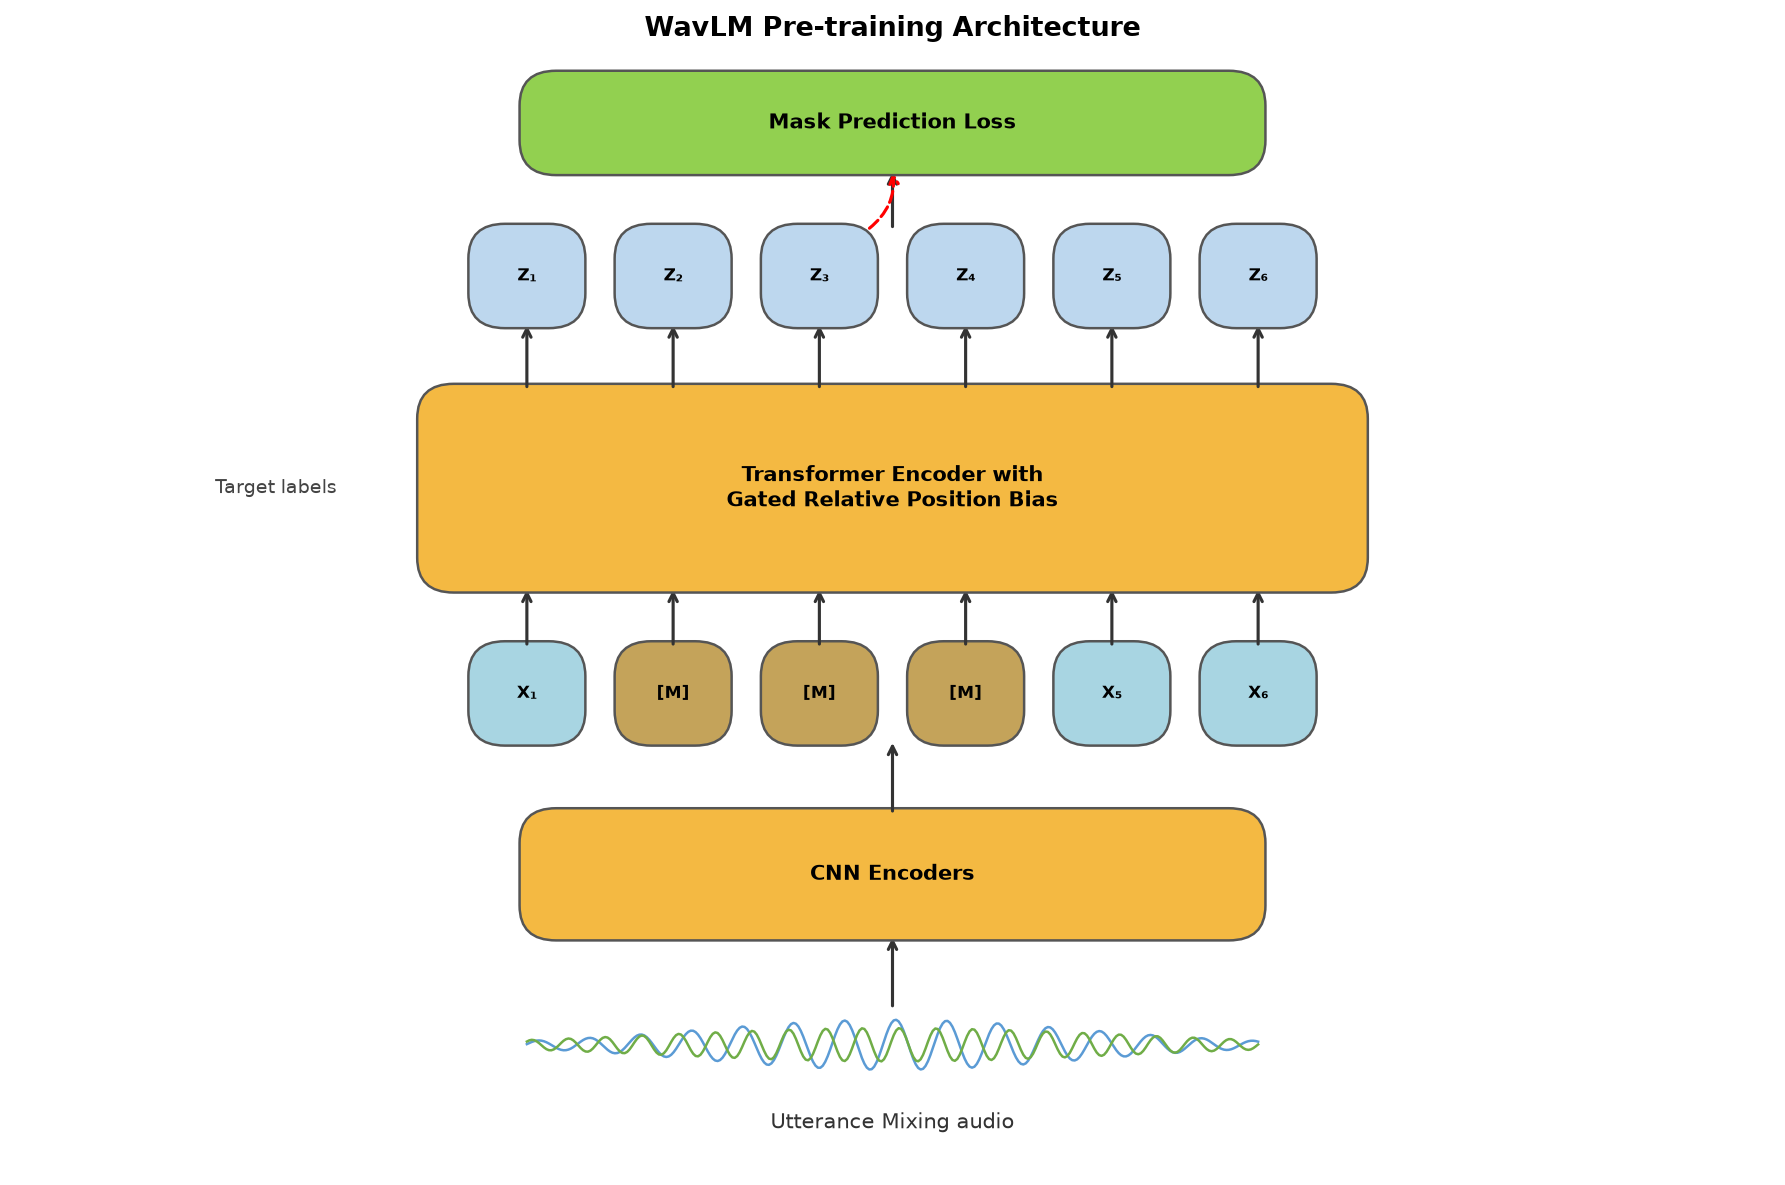
\includegraphics[width=0.60\linewidth]{figures/wavlm_architecture.png}
  \caption{WavLM pre-training architecture. CNN encoders extract local features
  from raw audio; the Transformer encoder with Gated Relative Position Bias
  contextualises them. A subset of frames is masked (\texttt{[M]}) and the model
  is trained to predict target representations $Z_i$ from context via Mask
  Prediction Loss \cite{chen2022wavlm}.}
  \label{fig:wavlm}
\end{figure}

\textbf{Whisper} \cite{radford2023whisper} is developed by OpenAI and trained on
680,000 hours of transcribed audio. Because its objective is transcription, it
learns phonetic and linguistic structure rather than raw acoustic properties---a
perspective directly relevant to deepfake detection \cite{kawa2023whisper}, since
synthetic speech often contains subtle phonetic irregularities that acoustic
models may overlook. Architecturally, Whisper follows an encoder-decoder design;
we discard the decoder entirely and use only the encoder, which also produces
\textbf{768-dimensional} embeddings \cite{radford2023whisper}. This dimensional
alignment with WavLM means no projection layer is needed between the two branches.
Together, WavLM and Whisper offer complementary views of the same signal---one
acoustic, one phonetic---which is the core idea behind our fusion approach
\cite{pan2024attentive,elkheir2025two}.

\begin{figure}[htbp]
  \centering
  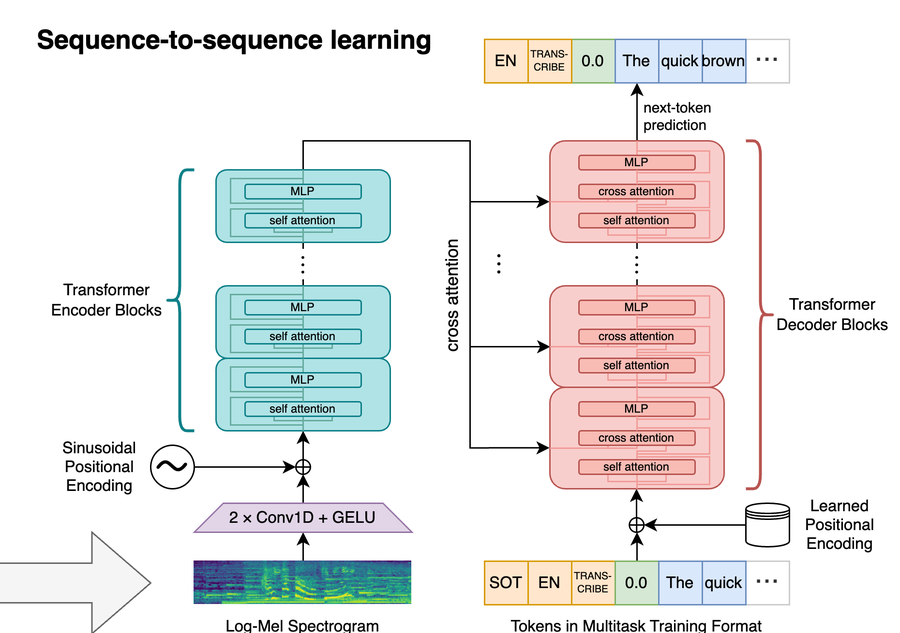
\includegraphics[width=0.85\linewidth]{figures/whisper_architecture.png}
  \caption{Whisper sequence-to-sequence architecture \cite{radford2023whisper}.
  The encoder (left, teal blocks) processes a Log-Mel Spectrogram through
  $2\!\times\!$Conv1D\,+\,GELU and stacked Transformer blocks. In
  FusionGuardNet only the encoder is used; the decoder (right, pink blocks) is
  discarded after feature extraction.}
  \label{fig:whisper}
\end{figure}

\subsection{Classification Architecture: Nes2Net}

Standard ResNet \cite{he2016resnet} introduced residual connections that allow
gradients to flow cleanly through deep networks. Res2Net \cite{gao2021res2net}
extended this by splitting feature channels into hierarchical subsets, enabling
multi-scale feature capture in a single forward pass---useful for audio because
spoofing artifacts appear at different time resolutions
\cite{li2021res2net,fan2023res2net}.

Nes2Net \cite{liu2025nes2net} (Liu et al., 2025) nests an additional residual
connection inside each Res2Net block, creating a two-level hierarchy of residual
pathways. An inner shortcut preserves fine-grained information while the outer one
propagates more abstract representations. Each block also incorporates a
Squeeze-and-Excitation (SE) module for channel-wise recalibration. A key practical
advantage is that Nes2Net accepts the high-dimensional output of speech foundation
models directly, without a dimensionality reduction step, followed by global
pooling and a linear classification head.

% ─────────────────────────────────────────────────────────────────────────────
\section{Dataset and Preprocessing}

\subsection{The Selected Datasets}

We conducted experiments on two dataset configurations of increasing scale.

\subsubsection{ASVspoof 2019 Logical Access (LA)}
ASVspoof 2019 LA \cite{kinnunen2019asvspoof} is one of the most widely adopted
benchmarks in speech anti-spoofing. It contains recordings from 19 different TTS
and VC algorithms alongside genuine speech collected in a controlled environment,
distributed in FLAC format with protocol files mapping utterance IDs to
bonafide/spoof labels and system identifiers.

\subsubsection{ASVspoof5 (2024)}
ASVspoof5 \cite{wang2024asvspoof5} is the most recent release in the series,
collected under more challenging and diverse conditions with a broader range of
modern synthesis systems. Including it alongside the 2019 data exposes the model
to a wider variety of spoofing artifacts, supporting better generalization.

\subsubsection{Fake-or-Real (for-norm subset)}
Fake-or-Real \cite{abdeldayem2024fakeorreal} is a publicly available dataset
comprising real recordings and AI-generated speech. We use only the
\texttt{for-norm} folder---studio-quality, noise-normalized samples---which
contributes approximately 69,300 samples to Dataset~2 ($\sim$34,650 real and
34,650 fake), adding diversity in recording conditions and synthesis methods not
present in the ASVspoof corpora.

\subsection{Dataset Configurations}

\begin{table}[htbp]
  \centering
  \caption{Dataset configurations used in this project.}
  \label{tab:datasets}
  \begin{tabularx}{\linewidth}{llX}
    \toprule
    Configuration & Name & Included datasets \\
    \midrule
    Dataset 1 & ASVspoof Combined (ASVsp-C) &
      ASVspoof 2019 LA + ASVspoof5 2024 \\
    Dataset 2 & ASVspoof-FoR Extended (ASVsp-FoR) &
      ASVspoof 2019 LA + ASVspoof5 2024 + Fake-or-Real (for-norm) \\
    \bottomrule
  \end{tabularx}
\end{table}

\subsection{Data Splitting}

After merging all entries, the pool is split into train, validation, and test sets
using an \textbf{80\,/\,10\,/\,10} ratio. Class balance is enforced independently
for real and fake entries, shuffled with random seed 42 for reproducibility.

\begin{table}[htbp]
  \centering
  \caption{Sample counts by dataset configuration, split, and class.}
  \label{tab:splits}
  \begin{tabular}{llrrr}
    \toprule
    Configuration & Split & Real & Fake & Total \\
    \midrule
    Dataset 1 & Train &  42,139 &  42,139 &  84,278 \\
    Dataset 1 & Dev   &   5,267 &   5,267 &  10,534 \\
    Dataset 1 & Test  &   5,268 &   5,268 &  10,536 \\
    \midrule
    Dataset 2 & Train &  69,823 &  69,895 & 139,718 \\
    Dataset 2 & Dev   &   8,727 &   8,736 &  17,463 \\
    Dataset 2 & Test  &   8,729 &   8,738 &  17,467 \\
    \bottomrule
  \end{tabular}
\end{table}

% ─────────────────────────────────────────────────────────────────────────────
\section{System Architecture and Proposed Methodology}

\subsection{End-to-End System Overview}

FusionGuardNet follows a three-stage pipeline with clear stage separation: (1)
offline feature extraction through frozen encoders, (2) learnable feature fusion,
and (3) Nes2Net classification. The two encoders are never fine-tuned; only the
fusion layer and backbone are trained.

\begin{figure}[htbp]
  \centering
  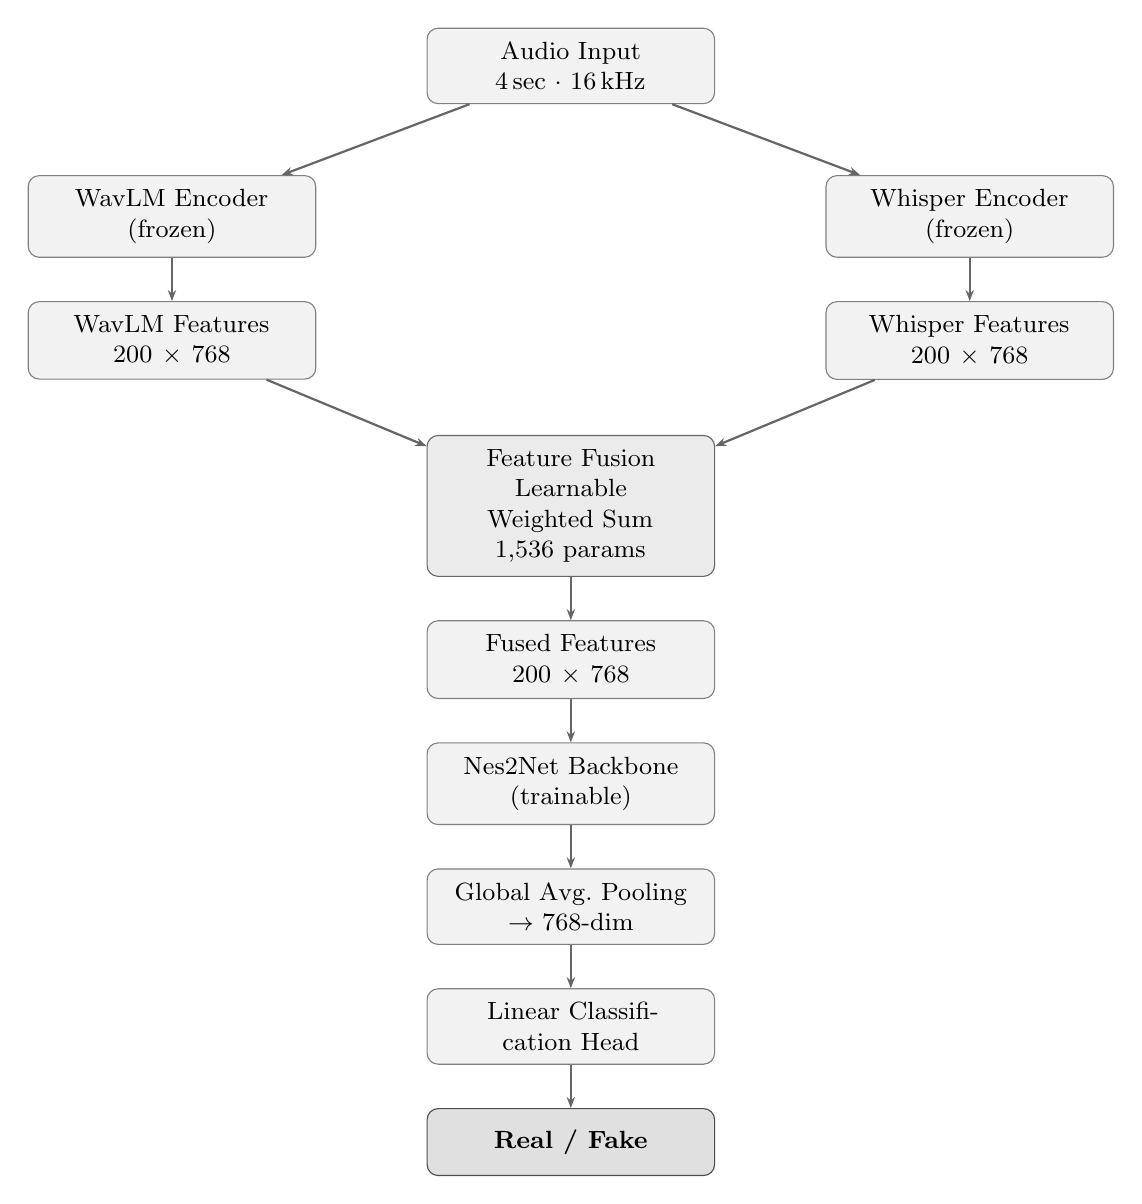
\begin{tikzpicture}[
    node distance=0.55cm and 2.2cm,
    every node/.style={font=\small},
    box/.style={rectangle, rounded corners=4pt, draw=black!50, fill=black!5,
                text width=3.3cm, align=center, minimum height=0.85cm, inner sep=5pt},
    gbox/.style={rectangle, rounded corners=4pt, draw=black!70, fill=black!12,
                text width=3.3cm, align=center, minimum height=0.85cm, inner sep=5pt,
                font=\small\bfseries},
    fbox/.style={rectangle, rounded corners=4pt, draw=black!60, fill=black!8,
                text width=3.3cm, align=center, minimum height=0.85cm, inner sep=5pt},
    arr/.style={-{Stealth[length=4pt]}, thick, black!60}
  ]
  \node[box] (audio) {Audio Input\\4\,sec $\cdot$ 16\,kHz};

  \node[box, below left=0.9cm and 1.4cm of audio]  (we)
        {WavLM Encoder\\(frozen)};
  \node[box, below right=0.9cm and 1.4cm of audio] (se)
        {Whisper Encoder\\(frozen)};

  \node[box, below=0.55cm of we] (wf) {WavLM Features\\$200\times768$};
  \node[box, below=0.55cm of se] (sf) {Whisper Features\\$200\times768$};

  \coordinate (mid) at ($(wf)!0.5!(sf)$);
  \node[fbox, below=1.2cm of mid] (fus)
        {Feature Fusion\\Learnable Weighted Sum\\1,536 params};

  \node[box, below=0.55cm of fus] (ff)  {Fused Features\\$200\times768$};
  \node[box, below=0.55cm of ff]  (n2n) {Nes2Net Backbone\\(trainable)};
  \node[box, below=0.55cm of n2n] (gap) {Global Avg.\ Pooling\\$\to$ 768-dim};
  \node[box, below=0.55cm of gap] (clf) {Linear Classification Head};
  \node[gbox, below=0.55cm of clf] (out) {Real / Fake};

  \draw[arr] (audio) -- (we);
  \draw[arr] (audio) -- (se);
  \draw[arr] (we)  -- (wf);
  \draw[arr] (se)  -- (sf);
  \draw[arr] (wf)  -- (fus);
  \draw[arr] (sf)  -- (fus);
  \draw[arr] (fus) -- (ff);
  \draw[arr] (ff)  -- (n2n);
  \draw[arr] (n2n) -- (gap);
  \draw[arr] (gap) -- (clf);
  \draw[arr] (clf) -- (out);
  \end{tikzpicture}
  \caption{FusionGuardNet end-to-end pipeline. The two frozen encoders extract
  complementary features; a learnable fusion layer combines them; the Nes2Net
  backbone classifies the result.}
  \label{fig:pipeline}
\end{figure}

\subsection{Audio Signal Preprocessing}

\begin{table}[htbp]
  \centering
  \caption{Audio preprocessing steps applied uniformly across all source datasets.}
  \label{tab:preproc}
  \begin{tabularx}{\linewidth}{lX}
    \toprule
    Step & Description \\
    \midrule
    Channel reduction         & Multi-channel recordings are averaged to mono. \\
    Sample rate normalization & Every waveform is resampled to 16,000\,Hz (Torchaudio). \\
    Fixed-length normalization & Normalized to exactly 4 seconds (64,000 samples).
                                 Longer clips are randomly cropped; shorter clips are
                                 zero-padded at the end. \\
    Padding-validity mask     & A frame-level binary mask marks real frames as 1 and
                                 padded frames as 0. \\
    \bottomrule
  \end{tabularx}
\end{table}

\subsection{Acoustic and Semantic Feature Extraction: WavLM and Whisper}

Both WavLM and Whisper representations are computed once for all clips and saved
as PyTorch tensor files (\texttt{.pt}), avoiding redundant forward passes through
large models during training.

\subsubsection{WavLM extraction}
The preprocessed 16\,kHz mono waveform is passed into the frozen
\texttt{microsoft/wavlm-base-plus} encoder, producing \textbf{768-dimensional}
frame-level embeddings at 20\,ms resolution. A 4-second clip yields
\textbf{200 frames}.

\subsubsection{Whisper extraction}
The waveform is first converted to an \textbf{80-band log-Mel spectrogram} and
passed through the frozen \texttt{openai/whisper-small} encoder (decoder
discarded). The encoder produces \textbf{768-dimensional} contextual embeddings
reflecting phonetic and prosodic structure.

\begin{figure}[htbp]
  \centering
  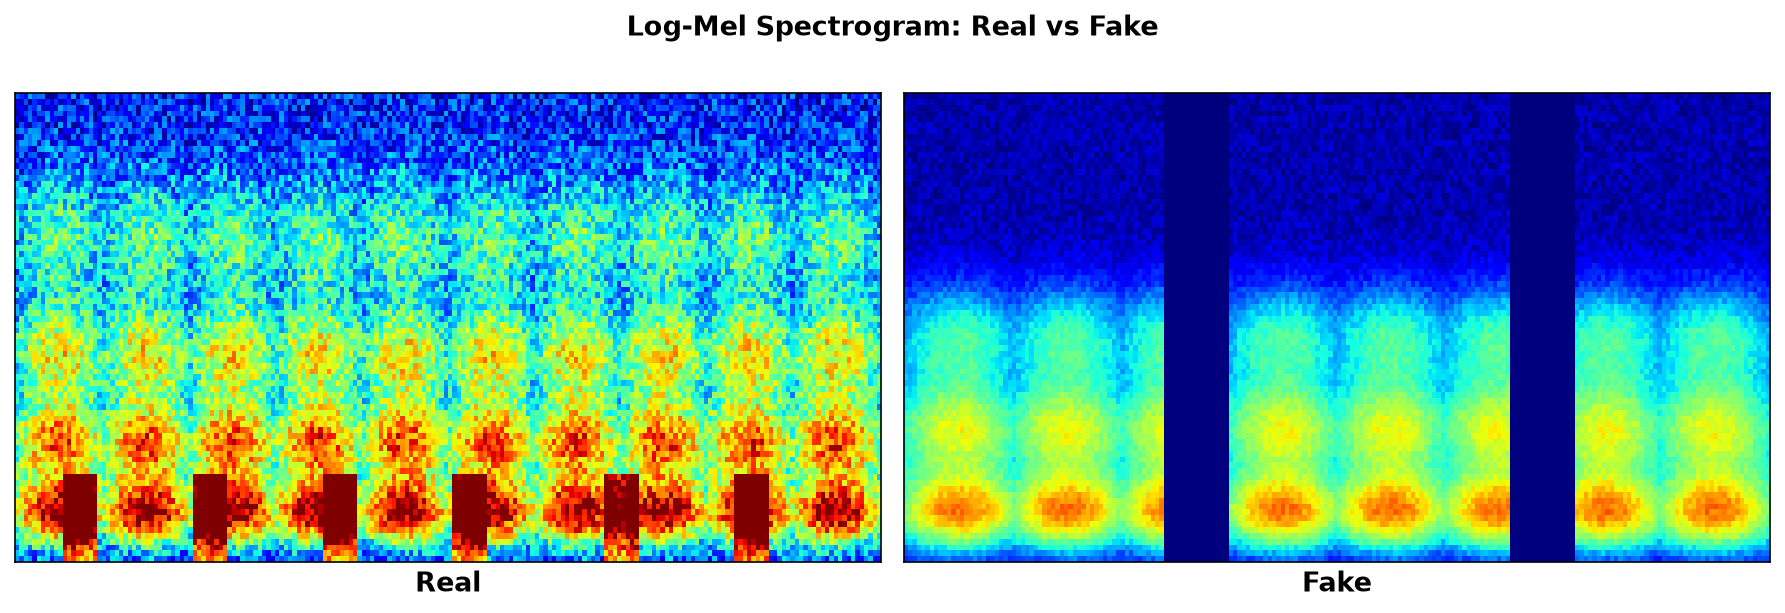
\includegraphics[width=0.84\linewidth]{figures/spectrogram_real_vs_fake.png}
  \caption{Log-Mel spectrogram comparison. Real speech (left) shows denser, more
  irregular low-frequency energy; synthetic speech (right) displays smoother,
  more uniform spectral structure with visible silence bands---differences that
  motivate the Whisper encoder branch.}
  \label{fig:spectro}
\end{figure}

\subsubsection{Temporal alignment}
WavLM and Whisper produce feature sequences of different temporal lengths for
the same 4-second input. The Whisper sequence is aligned to the WavLM sequence
length by truncation (if longer) or zero-padding at the end (if shorter), ensuring
a shared time axis for frame-by-frame fusion.

\subsection{Feature Fusion: Combining WavLM and Whisper}

The fusion module takes two aligned sequences of shape $T\times768$ and combines
them via a \textbf{learnable weighted sum}. Two weight vectors
$\boldsymbol{\alpha}_1, \boldsymbol{\alpha}_2 \in \mathbb{R}^{768}$ are learned;
before combining, they are passed through a softmax so the weights are positive
and sum to 1 at each feature dimension:
\begin{equation}
  \mathbf{f}_t = \boldsymbol{\sigma}_1 \odot \mathbf{w}_t \;+\;
                 \boldsymbol{\sigma}_2 \odot \mathbf{s}_t,
  \qquad
  [\boldsymbol{\sigma}_1, \boldsymbol{\sigma}_2]
  = \operatorname{softmax}([\boldsymbol{\alpha}_1, \boldsymbol{\alpha}_2])
  \label{eq:fusion}
\end{equation}
where $\mathbf{w}_t$ and $\mathbf{s}_t$ are the WavLM and Whisper embeddings at
time~$t$, and $\odot$ denotes element-wise multiplication. This adds only
$2\times768 = 1{,}536$ trainable parameters and is interpretable: the learned
weights reveal which model the classifier relies on per feature dimension.

\subsection{Classification Model: Adapting Nes2Net to the Fused Features}

The fused $T\times768$ sequence is passed directly to the Nes2Net backbone
without dimensionality reduction. After the stack of nested residual blocks,
global average pooling collapses the temporal dimension to a single 768-dim
vector, which is passed to a linear classification head producing two logits
(real/fake). During training, cross-entropy loss is applied; at inference, the
argmax determines the final prediction.

The NES ratio is $(8, 8)$ and dilation factor is 2, matching the original
Nes2Net configuration \cite{liu2025nes2net}. A dropout rate of 0.5 is applied
during training.

\subsection{Feature Dimensions and Architectural Comparison}

\begin{table}[htbp]
  \centering
  \caption{Tensor dimensions at each processing stage of FusionGuardNet.}
  \label{tab:dims}
  \begin{tabularx}{\linewidth}{lrX}
    \toprule
    Component & Output shape & Explanation \\
    \midrule
    Input audio              & 64,000 samples        & 4 sec at 16\,kHz \\
    WavLM features           & $200\times768$        & Frame-level, 20\,ms stride \\
    Whisper (pre-alignment)  & variable $\times768$  & Encoder embeddings from log-Mel \\
    Whisper (post-alignment) & $200\times768$        & Truncated or zero-padded \\
    Fusion input             & $2\times200\times768$ & WavLM + Whisper branches \\
    Fusion output            & $200\times768$        & Channel-wise weighted combination \\
    Fusion trainable params  & 1,536                 & 2 weight vectors of dim 768 \\
    Nes2Net input            & $200\times768$        & No projection layer required \\
    Global pooling output    & 768                   & Temporal axis collapsed \\
    Classification output    & 2 logits              & Real / Fake \\
    \bottomrule
  \end{tabularx}
\end{table}

% ─────────────────────────────────────────────────────────────────────────────
\section{Experimental Setup}

\subsection{Environment and Software Libraries}

All experiments were run on a CUDA-enabled GPU with automatic CPU fallback.
The project uses PyTorch as the main framework, Torchaudio for audio I/O, and
the Hugging Face Transformers library to load WavLM and Whisper. Additional
libraries include NumPy, Pandas, scikit-learn, Matplotlib, and Seaborn.

\subsection{Training Procedure}

Training used the Adam optimizer with learning rate $10^{-4}$ and weight decay
$10^{-4}$ (L2 regularization), cross-entropy loss, gradient clipping (max
norm~1.0), and a ReduceLROnPlateau scheduler that halves the learning rate when
validation loss stagnates for 2 consecutive epochs. Training ran for \textbf{8
epochs} with batch size \textbf{16} and early stopping (patience~4). The best
checkpoint was saved by combined validation accuracy and loss. Random seed was
fixed to 42 for reproducibility.

\subsection{Hyperparameter Configuration}

\begin{table}[htbp]
  \centering
  \caption{Hyperparameter configuration used for all training runs.}
  \label{tab:hparams}
  \begin{tabular}{lr}
    \toprule
    Hyperparameter & Value \\
    \midrule
    Input feature dimension  & 768 \\
    NES ratio                & (8, 8) \\
    Dilation factor          & 2 \\
    Dropout rate             & 0.5 \\
    Pooling                  & Global average pooling \\
    Audio sample rate        & 16,000\,Hz \\
    Audio duration           & 4 seconds \\
    Samples per clip         & 64,000 \\
    Temporal sequence length & 200 frames \\
    Fusion type              & Learnable weighted sum (softmax-normalised) \\
    WavLM variant            & \texttt{microsoft/wavlm-base-plus} \\
    Whisper variant          & \texttt{openai/whisper-small} \\
    Optimizer                & Adam \\
    Learning rate            & $10^{-4}$ \\
    Weight decay             & $10^{-4}$ \\
    Batch size               & 16 \\
    Max epochs               & 8 \\
    Early stopping patience  & 4 \\
    \bottomrule
  \end{tabular}
\end{table}

\subsection{Evaluation Metrics}

\begin{table}[htbp]
  \centering
  \caption{Evaluation metrics used in this project.}
  \label{tab:metrics}
  \begin{tabularx}{\linewidth}{lX}
    \toprule
    Metric & Purpose \\
    \midrule
    Accuracy           & Overall fraction of correctly classified samples. \\
    Cross-Entropy loss & Tracks convergence and overfitting. \\
    Precision          & Fraction of predicted fakes that are truly fake. \\
    Recall             & Fraction of actual fakes correctly detected. \\
    F1-score           & Harmonic mean of precision and recall. \\
    EER                & Operating point where false acceptance and false
                         rejection rates are equal; lower is better. \\
    \bottomrule
  \end{tabularx}
\end{table}

% ─────────────────────────────────────────────────────────────────────────────
\section{Results and Discussion}

\subsection{Baseline Model Performance: WavLM + Nes2Net}

The baseline uses WavLM representations fed directly to the Nes2Net classifier,
with no Whisper branch. This provides a controlled reference: the classification
objective and backbone are identical to the proposed model, so any performance
difference is attributable solely to the addition of Whisper-derived information.

\subsection{Enhanced Model Performance: WavLM + Whisper + Nes2Net}

The enhanced configuration integrates WavLM and Whisper representations before
classification, allowing the model to jointly consider low-level acoustic
signatures and higher-level phonetic-linguistic patterns.

\begin{table}[htbp]
  \centering
  \caption{Main quantitative results for FusionGuardNet (WavLM + Whisper + Nes2Net).}
  \label{tab:results}
  \begin{tabular}{lrrrrr}
    \toprule
    Experiment & Accuracy & Precision & Recall & F1-score & EER \\
    \midrule
    Dataset 1 & 99.18\% & 99.18\% & 99.18\% & 99.18\% & N/A \\
    Dataset 2 & 99.34\% & 99.12\% & 99.57\% & 99.35\% & 0.60\% \\
    \bottomrule
  \end{tabular}
\end{table}

For \textbf{Dataset~1} (84,278 train / 10,536 test), the model produced only
86 total mistakes with a perfectly symmetric error profile
(TN\,=\,5,225, FP\,=\,43, FN\,=\,43, TP\,=\,5,225). Training converged
stably over 8 epochs, from 92.60\% in epoch~1 to 99.49\% in epoch~8, with best
dev accuracy of 99.25\%.

\begin{figure}[htbp]
  \centering
  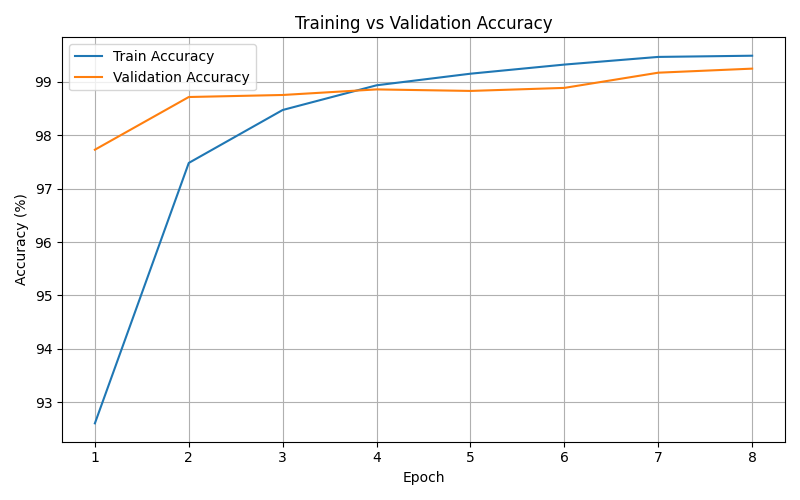
\includegraphics[width=0.74\linewidth]{results/results-d1/accuracy_curve.png}
  \caption{Dataset~1 --- Training vs.\ Validation Accuracy over 8 epochs.
  Stable convergence to 99.49\% training accuracy by epoch~8.}
  \label{fig:d1acc}
\end{figure}

\begin{figure}[htbp]
  \centering
  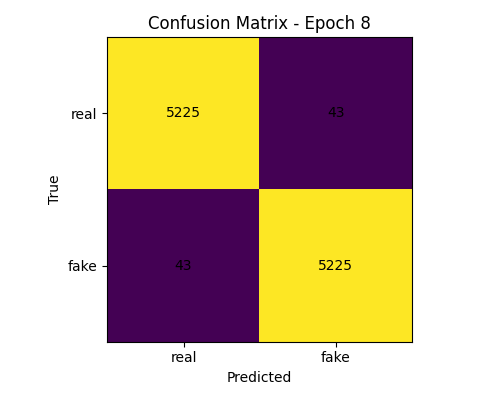
\includegraphics[width=0.62\linewidth]{results/results-d1/test_runs/test_epoch_08_2026-03-26_19-46-37/confusion_matrix_epoch_08.png}
  \caption{Dataset~1 --- Confusion Matrix (Epoch~8). Perfectly symmetric errors:
  43 false positives and 43 false negatives out of 10,536 test samples.}
  \label{fig:d1cm}
\end{figure}

For \textbf{Dataset~2} (139,718 train / 17,467 test), the system reached
99.34\% accuracy, 0.60\% EER, and confusion-matrix counts of
TN\,=\,8,652, FP\,=\,77, FN\,=\,38, TP\,=\,8,700.

\begin{figure}[htbp]
  \centering
  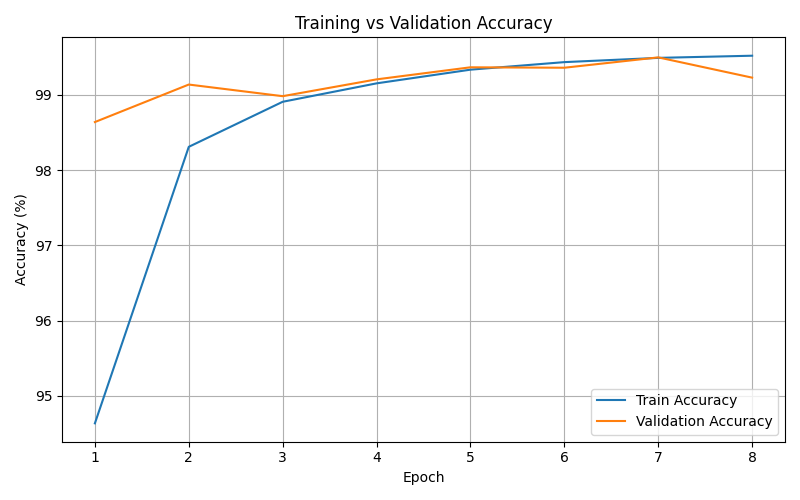
\includegraphics[width=0.74\linewidth]{results/results-d2/accuracy_curve.png}
  \caption{Dataset~2 --- Training vs.\ Validation Accuracy over 8 epochs.
  The fused model maintains stable convergence on the larger mixed-source dataset.}
  \label{fig:d2acc}
\end{figure}

\begin{figure}[htbp]
  \centering
  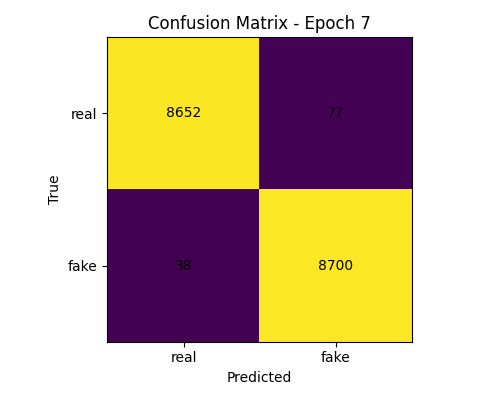
\includegraphics[width=0.62\linewidth]{results/results-d2/test_runs/test_epoch_07_2026-04-12_09-31-23/confusion_matrix_epoch_07.png}
  \caption{Dataset~2 --- Confusion Matrix (Epoch~7). TN\,=\,8,652, FP\,=\,77,
  FN\,=\,38, TP\,=\,8,700 across 17,467 test samples.}
  \label{fig:d2cm}
\end{figure}

\begin{figure}[htbp]
  \centering
  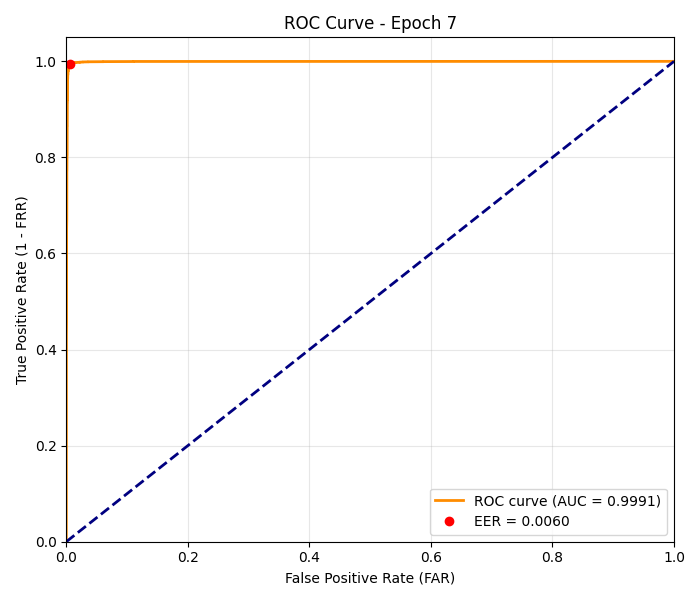
\includegraphics[width=0.74\linewidth]{results/results-d2/test_runs/test_epoch_07_2026-04-12_09-31-23/roc_curve_epoch_07.png}
  \caption{Dataset~2 --- ROC Curve (AUC\,=\,0.9991, EER\,=\,0.60\%, Epoch~7).
  Near-perfect discrimination across all operating thresholds.}
  \label{fig:d2roc}
\end{figure}

\subsection{Ablation Study: Relative Contribution of Whisper Integration}

\begin{table}[htbp]
  \centering
  \caption{Ablation study: baseline vs.\ proposed model.}
  \label{tab:ablation}
  \begin{tabular}{lll}
    \toprule
    Setting & Feature source & Classifier \\
    \midrule
    Baseline       & WavLM only      & Nes2Net \\
    Proposed model & WavLM + Whisper & Nes2Net \\
    \bottomrule
  \end{tabular}
\end{table}

Because both settings keep the same classifier family and objective, the main
changing factor is the addition of Whisper-derived information, making it possible
to attribute robustness gains cleanly to multimodal feature integration.

\subsection{Error Analysis}

In Dataset~1 the error profile is perfectly symmetric (FP\,=\,FN\,=\,43). In
Dataset~2 it is slightly asymmetric (FP\,=\,77, FN\,=\,38) but strongly balanced
relative to dataset size, indicating the model does not strongly favour either
class. Most mistakes cluster near the decision boundary or represent genuinely
hard synthesis artifacts that confuse both branches. This points toward two
practical improvements: (1) calibration-oriented techniques to reduce
overconfident mistakes; (2) targeted data expansion for borderline cases.

% ─────────────────────────────────────────────────────────────────────────────
\section{Conclusion and Future Work}

\subsection{Summary of Achievements}

FusionGuardNet implements a complete audio deepfake detection pipeline based on
feature-level integration of WavLM and Whisper, followed by a Nes2Net classifier.
Both encoders remain frozen; only the 1,536-parameter fusion layer and the
backbone are trained. The system achieves over 99\% accuracy on both dataset
configurations, with a balanced error profile and strong EER, validating the
hypothesis that acoustic\,+\,phonetic fusion yields a more robust detector than
either modality alone.

\subsection{Future Research Directions}

\begin{itemize}[noitemsep]
  \item \textbf{Full baseline suite}: run WavLM-only and Whisper-only settings
        with identical reporting to directly quantify each branch's contribution.
  \item \textbf{Robustness evaluation} on additional datasets and unseen
        synthesis methods to assess generalization under distribution shift.
  \item \textbf{Richer fusion strategies}: attention-based or cross-modal
        attention fusion instead of the current weighted sum.
  \item \textbf{Calibration methods} to reduce overconfident mistakes on
        borderline samples.
  \item \textbf{Lightweight inference} for near-real-time screening in
        production pipelines.
  \item \textbf{Interpretability analysis} of time-frequency regions to support
        explanation and diagnosis of failure modes.
\end{itemize}

% ─────────────────────────────────────────────────────────────────────────────
\begin{thebibliography}{39}

\bibitem{li2024survey}
Li, M., Ahmadiadli, Y., \& Zhang, X.-P. (2024).
\textit{A Survey on Speech Deepfake Detection}. arXiv:2404.13914.
\url{https://arxiv.org/abs/2404.13914}

\bibitem{yi2023survey}
Yi, J., Wang, C., Tao, J., Zhang, X., Zhang, C.~Y., \& Zhao, Y. (2023).
\textit{Audio deepfake detection: A survey}. arXiv:2308.14970.
\url{https://arxiv.org/abs/2308.14970}

\bibitem{li2025where}
Li, X., Chen, P.-Y., \& Wei, W. (2025).
\textit{Where are we in audio deepfake detection?}
ACM Transactions on Internet Technology, 25(3).
\url{https://arxiv.org/abs/2410.04324}

\bibitem{hong2026vulnerabilities}
Hong, M., Jiang, D., Xie, Z., Zhao, W., Wang, G., \& Zhang, C.~J. (2026).
\textit{Vulnerabilities of audio-based biometric authentication systems against
deepfake speech synthesis}. arXiv:2601.02914.
\url{https://arxiv.org/abs/2601.02914}

\bibitem{kamel2025survey}
Kamel, K., Sood, K., Sankar~Dutta, H., \& Aryal, S. (2025).
\textit{A survey of threats against voice authentication and anti-spoofing
systems}. arXiv:2508.16843.
\url{https://arxiv.org/abs/2508.16843}

\bibitem{chandra2025deepfake}
Chandra, N.~A., et al. (2025).
\textit{Deepfake-Eval-2024: A multi-modal in-the-wild benchmark}.
arXiv:2503.02857.
\url{https://arxiv.org/abs/2503.02857}

\bibitem{kinnunen2019asvspoof}
Kinnunen, T., Yamagishi, J., Todisco, M., Delgado, H., Sahidullah, M.,
Wang, W., Evans, N., \& Lee, K.~A. (2019).
\textit{ASVspoof 2019: Future horizons in spoofed and fake audio detection}.
In \textit{Proc.\ Interspeech 2019}, 1008--1012.
\url{https://arxiv.org/abs/1904.05441}

\bibitem{wang2024asvspoof5}
Wang, X., et al. (2024).
\textit{ASVspoof~5: Crowdsourced speech data, deepfakes, and adversarial
attacks at scale}.
In \textit{Proc.\ ASVspoof 2024 Workshop}.
\url{https://arxiv.org/abs/2408.08739}

\bibitem{liu2023asvspoof2021}
Liu, X., et al. (2023).
\textit{ASVspoof 2021: Towards spoofed and deepfake speech detection in the wild}.
IEEE/ACM Transactions on Audio, Speech, and Language Processing, 31, 2507--2522.
\url{https://arxiv.org/abs/2210.02437}

\bibitem{todisco2017cqcc}
Todisco, M., Delgado, H., \& Evans, N. (2017).
\textit{Constant Q cepstral coefficients: A spoofing countermeasure for
automatic speaker verification}.
Computer Speech \& Language, 45, 516--535.
\url{https://doi.org/10.1016/j.csl.2017.01.001}

\bibitem{muller2024harder}
Muller, N.~M., Evans, N., Tak, H., Sperl, P., \& Bottinger, K. (2024).
\textit{Harder or different? Understanding generalization of audio deepfake detection}.
In \textit{Proc.\ Interspeech 2024}.
\url{https://arxiv.org/abs/2406.03512}

\bibitem{nguyen2025linguistic}
Nguyen, B., Shi, S., Ofman, R., \& Le, T. (2025).
\textit{What you read isn't what you hear: Linguistic sensitivity in deepfake
speech detection}. arXiv:2505.17513.
\url{https://arxiv.org/abs/2505.17513}

\bibitem{zhu2024slim}
Zhu, Y., Koppisetti, S., Tran, T., \& Bharaj, G. (2024).
\textit{SLIM: Style-linguistics mismatch model for generalized audio deepfake detection}.
In \textit{Advances in NeurIPS~37}.
\url{https://arxiv.org/abs/2407.18517}

\bibitem{shi2025benchmarking}
Shi, H., Shi, X., Dogan, S., Alzubi, S., Huang, T., \& Zhang, Y. (2025).
\textit{Benchmarking audio deepfake detection robustness in real-world
communication scenarios}. arXiv:2504.12423.
\url{https://arxiv.org/abs/2504.12423}

\bibitem{chen2022wavlm}
Chen, S., Wang, C., Chen, Z., Wu, Y., Liu, S., et al. (2022).
\textit{WavLM: Large-scale self-supervised pre-training for full stack speech processing}.
IEEE Journal of Selected Topics in Signal Processing, 16(6), 1505--1518.
\url{https://arxiv.org/abs/2110.13900}

\bibitem{radford2023whisper}
Radford, A., Kim, J.~W., Xu, T., Brockman, G., McLeavey, C., \& Sutskever, I. (2023).
\textit{Robust speech recognition via large-scale weak supervision}.
In \textit{Proc.\ ICML 2023}, 28492--28518.
\url{https://arxiv.org/abs/2212.04356}

\bibitem{yang2021superb}
Yang, S.-W., Chi, P.-H., Chuang, Y.-S., et al. (2021).
\textit{SUPERB: Speech processing universal performance benchmark}.
In \textit{Proc.\ Interspeech 2021}, 1194--1198.
\url{https://arxiv.org/abs/2105.01051}

\bibitem{elkheir2025comprehensive}
El~Kheir, Y., Samih, Y., Maharjan, S., Polzehl, T., \& Moller, S. (2025).
\textit{Comprehensive layer-wise analysis of SSL models for audio deepfake detection}.
In \textit{Findings of ACL: NAACL 2025}, 4070--4082.
\url{https://arxiv.org/abs/2502.03559}

\bibitem{guo2024wavlm}
Guo, Y., Huang, H., Chen, X., Zhao, H., \& Wang, Y. (2024).
\textit{Audio deepfake detection with self-supervised WavLM and multi-fusion attentive classifier}.
In \textit{Proc.\ ICASSP 2024}, 12702--12706.
\url{https://arxiv.org/abs/2312.08089}

\bibitem{combei2024wavlm}
Combei, D., Stan, A., Oneata, D., \& Cucu, H. (2024).
\textit{WavLM model ensemble for audio deepfake detection}.
In \textit{Proc.\ ASVspoof 2024 Workshop}, 170--175.
\url{https://arxiv.org/abs/2408.07414}

\bibitem{stourbe2024wavlm}
Stourbe, T., Miara, V., Lepage, T., \& Dehak, R. (2024).
\textit{Exploring WavLM back-ends for speech spoofing and deepfake detection}.
In \textit{Proc.\ ASVspoof 2024 Workshop}, 72--78.
\url{https://arxiv.org/abs/2409.05032}

\bibitem{abdeldayem2024fakeorreal}
Abdel~Dayem, M. (n.d.).
\textit{The Fake-or-Real Dataset}. Kaggle.
\url{https://www.kaggle.com/datasets/mohammedabdeldayem/the-fake-or-real-dataset}

\bibitem{pan2024attentive}
Pan, Z., Liu, T., Sailor, H.~B., \& Wang, Q. (2024).
\textit{Attentive merging of hidden embeddings from pre-trained speech model for
anti-spoofing detection}.
In \textit{Proc.\ Interspeech 2024}.
\url{https://arxiv.org/abs/2406.10283}

\bibitem{elkheir2025two}
El~Kheir, Y., Das, A., Erdogan, E.~E., et al. (2025).
\textit{Two views, one truth: Spectral and self-supervised features fusion for
robust speech deepfake detection}. arXiv:2507.20417.
\url{https://arxiv.org/abs/2507.20417}

\bibitem{ahmadiadli2025beyond}
Ahmadiadli, Y., Zhang, X.-P., \& Khan, N. (2025).
\textit{Beyond identity: A generalizable approach for deepfake audio detection}.
arXiv:2505.06766.
\url{https://arxiv.org/abs/2505.06766}

\bibitem{baevski2020wav2vec}
Baevski, A., Zhou, H., Mohamed, A., \& Auli, M. (2020).
\textit{wav2vec~2.0: A framework for self-supervised learning of speech representations}.
In \textit{Advances in NeurIPS~33}, 12449--12460.
\url{https://arxiv.org/abs/2006.11477}

\bibitem{hsu2021hubert}
Hsu, W.-N., Bolte, B., Tsai, Y.-H.~H., Lakhotia, K., Salakhutdinov, R.,
\& Mohamed, A. (2021).
\textit{HuBERT: Self-supervised speech representation learning by masked
prediction of hidden units}.
IEEE/ACM Transactions on Audio, Speech, and Language Processing, 29, 3451--3460.
\url{https://arxiv.org/abs/2106.07447}

\bibitem{kawa2023whisper}
Kawa, P., Plata, M., Czuba, M., Szymanski, P., \& Syga, P. (2023).
\textit{Improved DeepFake detection using Whisper features}.
In \textit{Proc.\ Interspeech 2023}, 4009--4013.
\url{https://arxiv.org/abs/2306.01428}

\bibitem{he2016resnet}
He, K., Zhang, X., Ren, S., \& Sun, J. (2016).
\textit{Deep residual learning for image recognition}.
In \textit{Proc.\ CVPR 2016}, 770--778.
\url{https://arxiv.org/abs/1512.03385}

\bibitem{gao2021res2net}
Gao, S.-H., Cheng, M.-M., Zhao, K., Zhang, X.-Y., Yang, M.-H.,
\& Torr, P.~H.~S. (2021).
\textit{Res2Net: A new multi-scale backbone architecture}.
IEEE Transactions on PAMI, 43(2), 652--662.
\url{https://arxiv.org/abs/1904.01169}

\bibitem{li2021res2net}
Li, X., Li, N., Weng, C., Liu, X., Su, D., Yu, D., \& Meng, H. (2021).
\textit{Replay and synthetic speech detection with Res2Net architecture}.
In \textit{Proc.\ ICASSP 2021}, 6354--6358.
\url{https://arxiv.org/abs/2010.15006}

\bibitem{fan2023res2net}
Fan, C., Xue, J., Tao, J., Yi, J., Wang, C., Zheng, C., \& Lv, Z. (2023).
\textit{Spatial reconstructed local attention Res2Net with F0 subband for fake
speech detection}. arXiv:2308.09944.
\url{https://arxiv.org/abs/2308.09944}

\bibitem{liu2025nes2net}
Liu, T., Truong, D.~T., Das, R.~K., Lee, K.~A., \& Li, H. (2025).
\textit{Nes2Net: A lightweight nested architecture for foundation model driven
speech anti-spoofing}. arXiv:2504.05657.
\url{https://arxiv.org/abs/2504.05657}

\bibitem{huang2025sharpness}
Huang, W., Liu, X., Wang, X., Yamagishi, J., \& Qian, Y. (2025).
\textit{From sharpness to better generalization for speech deepfake detection}.
In \textit{Proc.\ Interspeech 2025}.
\url{https://arxiv.org/abs/2506.11532}

\bibitem{kang2024wav2vec}
Kang, T., Han, S., Choi, S., Seo, J., Chung, S., Lee, S., Oh, S.,
\& Kwak, I.-Y. (2024).
\textit{Experimental study: Enhancing voice spoofing detection models with wav2vec~2.0}.
arXiv:2402.17127.
\url{https://arxiv.org/abs/2402.17127}

\bibitem{zhang2024aasist2}
Zhang, Y., Lu, J., Shang, Z., Wang, W., \& Zhang, P. (2024).
\textit{Improving short utterance anti-spoofing with AASIST2}.
In \textit{Proc.\ ICASSP 2024}.
\url{https://arxiv.org/abs/2309.08279}

\bibitem{wu2024codecfake}
Wu, H., Tseng, Y., \& Lee, H.-y. (2024).
\textit{CodecFake: Enhancing anti-spoofing models against deepfake audios from
codec-based speech synthesis systems}.
In \textit{Proc.\ Interspeech 2024}, 1770--1774.
\url{https://arxiv.org/abs/2406.07237}

\bibitem{pascu2024calibrated}
Pascu, O., Stan, A., Oneata, D., Oneata, E., \& Cucu, H. (2024).
\textit{Towards generalisable and calibrated audio deepfake detection with
self-supervised representations}.
In \textit{Proc.\ Interspeech 2024}, 4828--4832.
\url{https://www.isca-archive.org/interspeech_2024/pascu24_interspeech.html}

\bibitem{lopez2025generalizable}
Lopez, J.~A., Stemmer, G., \& Cordourier~Maruri, H. (2025).
\textit{Generalizable detection of audio deepfakes}. arXiv:2507.01750.
\url{https://arxiv.org/abs/2507.01750}

\end{thebibliography}

% ─────────────────────────────────────────────────────────────────────────────
\appendix
\section{Glossary}

\begin{description}[style=nextline, leftmargin=3cm, labelwidth=2.8cm,
                    font=\normalfont\bfseries]
  \item[Anti-spoofing] Automatically detecting whether a given audio sample is
    genuine speech or a synthetically generated/modified recording designed to
    deceive an authentication system.
  \item[ASVspoof] A challenge series and dataset collection providing standardized
    benchmarks for automatic speaker verification anti-spoofing research, running
    since 2015.
  \item[Bonafide] Term used in ASVspoof datasets to label authentic, real human
    speech samples (as opposed to spoofed samples).
  \item[Cross-Entropy Loss] Standard loss function for classification tasks
    measuring the difference between a predicted probability distribution and the
    true label distribution.
  \item[EER] Equal Error Rate---a threshold-independent metric for binary
    classifiers measuring the operating point at which false acceptance and false
    rejection rates are equal; lower is better.
  \item[Embedding] A dense, high-dimensional numerical vector produced by encoding
    an audio frame or utterance through a neural model.
  \item[Feature Fusion] Combining feature representations from multiple sources
    (here, WavLM and Whisper) into a single unified representation before
    classification.
  \item[FLAC] Free Lossless Audio Codec; lossless audio compression format used
    by ASVspoof 2019 and ASVspoof5 datasets.
  \item[HuBERT] Hidden-Unit BERT; a self-supervised speech model from Meta AI
    that learns representations by predicting discrete cluster assignments for
    masked audio frames.
  \item[Log-Mel Spectrogram] A 2-D time-frequency representation of audio where
    the frequency axis is Mel-scaled and pixel intensity represents log-energy;
    the standard input format for Whisper.
  \item[Nes2Net] Nested Res2Net; a lightweight backbone for speech anti-spoofing
    that nests an inner residual shortcut inside each Res2Net block.
  \item[Offline Feature Extraction] A pipeline strategy where large model
    inference is performed once before training and results are saved to disk.
  \item[Precision] Fraction of predicted-positive (fake) samples that are truly
    positive. High precision means few false alarms.
  \item[Pre-trained Model] A neural model trained on a large external dataset
    whose learned weights are reused for a downstream task.
  \item[Recall] Fraction of actual positive (fake) samples correctly identified.
    High recall means few missed detections.
  \item[Res2Net] A backbone architecture capturing features at multiple
    granularities within a single residual block via hierarchical channel splits.
\end{description}

\end{document}
